
\documentclass[11pt]{article}

\usepackage{alltt,fullpage,epsfig,amsmath,amssymb,subfig}
\usepackage[table]{xcolor} 

\usepackage{listings}
\lstset{
  breaklines=true,
  keepspaces=true,
  numbers=left
}

\newcommand{\auth}{Lisa Li \& Nate Brennand}
\newcommand{\class}{COMS 4112 - Project \#2}


\usepackage{fancyhdr}
\fancypagestyle{plain}{
  \fancyhf{}% Clear header/footer
  \fancyhead[L]{\auth}
  \fancyhead[R]{\class}
}
\pagestyle{plain}% Set page style to plain.

\author{\auth}
\title{\class}


\begin{document}
\setlength{\parskip}{.1 in}

\maketitle
\newpage

\section*{Introduction}

In this report, we focus on the results obtained from running our build algorithm on varying values for B (the size of the bucket), h (number of hash functions) and R (the number reinsertions allowed).
The values of B chosen consisted of: 1, 2, 4, 8; the values of h were: 2, 3, 4, 8; the values of R were: 1, 5, 20, 100, 1000.
As a control, we used the same S = 12 (size of table) for each table.
The full tables (Tables 7-10) displaying the results of each permutation of B, h and R are at the end of this report.

\section*{Evaluation}

\subsection*{Failure Thresholds}
To determine at what level the splash table is able to be filled before failure occurs, we generated the load factors for 20 build attempts for each combination of B and h.
For the purposes of this section, we considered splash tables when R = 1000.
For most combinations of B and h, the average load factor remained at a high percentage.
Of the 12 combinations displayed in the table above, 75\% of these combinations resulted in splash tables that were over 90\% full.
However, for the splash table where B = 1 and h = 2, we noticed that the average load factor was particularly low at only a little above 50\% full.

Compared to the failure load rates in the reference paper, our values were smaller, though still within a close range. Reasons for this variation can include differing implemenetations of algorithms being run, including the language used, as well as different specifications of the devices these were evaluated on. 

\begin{table}
\parbox{.45\linewidth}{
\centering
\small
\begin{tabular}{|l|l|l|}
\hline
\textbf{B} & \textbf{h} & \textbf{Average Load Factor} \\ \hline
1          & 2                 &0.51864015 \\ \hline
1          & 3                &0.9043823 \\ \hline
1          & 4           &0.9692871 \\ \hline
1          & 8               &0.9988037 \\ \hline
\rowcolor{gray!50}2          & 2           &0.72716065 \\ \hline
2          & 3                 &0.9599365 \\ \hline
2          & 4               &0.99046635 \\ \hline
2          & 8                &0.99968275 \\ \hline
\rowcolor{gray!50}4          & 2              &0.84698495 \\ \hline
\rowcolor{gray!50}4          & 3             &0.9828735 \\ \hline
\rowcolor{gray!50}4          & 4               &0.99570315 \\ \hline
4          & 8             &0.9999512 \\ \hline
\rowcolor{gray!50}8          & 2                &0.9267822 \\ \hline
8          & 3              &0.99177255 \\ \hline
8          & 4             &0.99796145 \\ \hline
8          & 8               &0.9999878 \\ \hline
\end{tabular}
\caption{Failure thresholds for varying choices of B and h.}}
\hfill
\parbox{.45\linewidth}{
\centering
\small
\begin{tabular}{|l|l|l|}
\hline
\textbf{B} & \textbf{h} & \textbf{Average Load Factor} \\ \hline
2          & 2            &0.89 \\ \hline
4          & 2            &0.976 \\ \hline
4          & 3            &0.998 \\ \hline
4          & 4            &0.997 \\ \hline
8 			&2 				&0.997 \\ \hline
\end{tabular}
\caption{Failure thresholds from reference paper}}
\end{table}

\subsection*{Variation in R}

\begin{figure}
\centering
\begin{tabular}{ccc}
\subfloat[B=1]{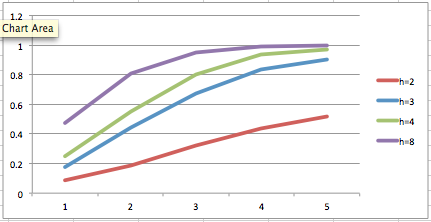
\includegraphics[scale=0.5]{b1}} &
\subfloat[B=2]{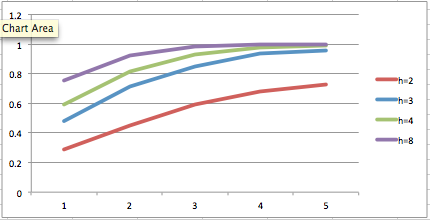
\includegraphics[scale=0.5]{b2}} \\
\subfloat[B=4]{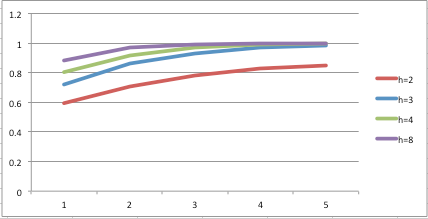
\includegraphics[scale=0.5]{b3}} &
\subfloat[B=8]{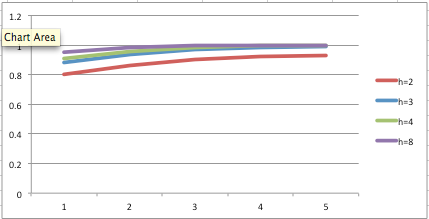
\includegraphics[scale=0.5]{b4}}
\end{tabular}
\caption{Variations in R}
\label{fig6}
\end{figure}

In this report, we used the values of 1, 5, 20, 100 and 1000 for R to see if we could evaluate the importance of choosing R in creating this splash table. 
For every instance of B and h, as the value of R increased, the average load factor displayed a marked increase as well.
This data seems to correlate with expected results, in that as the number of reinsertions increases, the amount of keys that are able to be successfully inserted into the splash table increases as well, and the probability that the build will succeed is established. 
The largest increase in average load factors was displayed from R=1 to R=5, with following increases to R resulting in a smaller change in average load factor, even as R jumped from 100 to 1000.
As such, we can conclude that while the number of reinsertions plays an important role in determining whether a build is ultimately successful, the increase in average load factor minimizes with subsequent increases in R. 

\subsection*{Importance of Varying Factors}
We compared the splash tables by their value for h, assumimg B and R remained the same, and noticed as that the number of hash functions generated for each key increased, the more successful entries into the splash table were made.
Similarly, we saw that an increase in the number of entries in a bucket also resulted in an increase in the average load factor for a splash table, assumimg R and h remained the same for each table. 

\begin{table}
\parbox{.45\linewidth}{
\centering
\small
\begin{tabular}{|l|l|l|}
\hline
\textbf{B} & \textbf{h} & \textbf{Average Load Factor} \\ \hline
1          & 2              &0.51864015 \\ \hline
1          & 3                 &0.9043823 \\ \hline
1          & 4             &0.9692871 \\ \hline
1          & 8                 &0.9988037 \\ \hline
\end{tabular}
\caption{Impact of h with B=1 and R=1000}}
\hfill
\parbox{.45\linewidth}{
\centering
\small
\begin{tabular}{|l|l|l|}
\hline
\textbf{B} & \textbf{h} & \textbf{Average Load Factor} \\ \hline
1          & 2            &0.51864015 \\ \hline
2          & 2            &0.72716065 \\ \hline
4          & 2            &0.84698495 \\ \hline
8          & 2            &0.9267822 \\ \hline
\end{tabular}
\caption{Impact of B with h=2 and R=1000}}
\end{table}

With an increase in h, fewer reinsertions are needed in order to place a key into the table, and as the bucket size increases, more keys are able to be placed in the same bucket. 
For most cases, an increase in the number of hash functions has a greater impact on the average load factor than an increase in the number of reinsertions.
The change in average load rate as R increases is smaller than the change in average load rate as h increases, even at the greatest jump for R (as R goes from 1 to 5).

\begin{table}
\parbox{.45\linewidth}{
\centering
\small
\begin{tabular}{|l|l|l|l|}
\hline
\textbf{B} & \textbf{h}  &\textbf{R} &\textbf{Average Load Factor} \\ \hline
1          & 2          & 1        &0.0869628 \\ \hline
1          & 2          & 5        &0.1856445 \\ \hline
1          & 4          & 1        &0.2493895 \\ \hline
\end{tabular}
\caption{Comparing h and R}
}
\hfill
\parbox{.45\linewidth}{
\centering
\small
\begin{tabular}{|l|l|l|l|}
\hline
\textbf{B} & \textbf{h}  &\textbf{R} &\textbf{Average Load Factor} \\ \hline
2          & 4          & 5        &0.8130494 \\ \hline
2          & 4          & 20        &0.9279907 \\ \hline
2          & 8          & 5        &0.9261597 \\ \hline
\end{tabular}
\caption{Comparing h and R}
}
\end{table}

\begin{table}
\parbox{.45\linewidth}{
\centering
\small
\begin{tabular}{|l|l|l|l|}
\hline
\textbf{B} & \textbf{h} & \textbf{R} & \textbf{Average Load Factor}\\ \hline
1          & 2          & 1        &0.0869628 \\ \hline
1          & 2          & 5        &0.1856445 \\ \hline
1          & 2          & 20        &0.3246338 \\ \hline
1          & 2          & 100        &0.43833 \\ \hline
1          & 2          & 1000        &0.51864015 \\ \hline
1          & 3          & 1        &0.1761718 \\ \hline
1          & 3          & 5        &0.44554435 \\ \hline
1          & 3          & 20        &0.6700195 \\ \hline
1          & 3          & 100        &0.83254395 \\ \hline
1          & 3          & 1000        &0.9043823 \\ \hline
1          & 4          & 1        &0.2493895 \\ \hline
1          & 4          & 5        &0.55366205 \\ \hline
1          & 4          & 20        &0.7990234 \\ \hline
1          & 4          & 100        &0.934607 \\ \hline
1          & 4          & 1000        &0.9692871 \\ \hline
1          & 8          & 1        &0.4738525 \\ \hline
1          & 8          & 5        &0.8066039 \\ \hline
1          & 8          & 20        &0.94992675 \\ \hline
1          & 8          & 100        &0.98983155 \\ \hline
1          & 8          & 1000        &0.9988037 \\ \hline
\end{tabular}
\caption{Results for B=1}
}
\hfill
\parbox{.45\linewidth}{
\centering
\small
\begin{tabular}{|l|l|l|l|}
\hline
\textbf{B} & \textbf{h} & \textbf{R} & \textbf{Average Load Factor} \\ \hline
2          & 2          & 1        &0.2883546 \\ \hline
2          & 2          & 5        &0.4511963 \\ \hline
2          & 2          & 20        &0.5919312 \\ \hline
2          & 2          & 100        &0.68099365 \\ \hline
2          & 2          & 1000        &0.72716065 \\ \hline
2          & 3          & 1        &0.4800782 \\ \hline
2          & 3          & 5        &0.712207 \\ \hline
2          & 3          & 20        &0.85026855 \\ \hline
2          & 3          & 100        &0.93522945 \\ \hline
2          & 3          & 1000        &0.9599365 \\ \hline
2          & 4          & 1        &0.5903565 \\ \hline
2          & 4          & 5        &0.8130494 \\ \hline
2          & 4          & 20        &0.9279907 \\ \hline
2          & 4          & 100        &0.9755737 \\ \hline
2          & 4          & 1000        &0.99046635 \\ \hline
2          & 8          & 1        &0.752234 \\ \hline
2          & 8          & 5        &0.9261597 \\ \hline
2          & 8          & 20        &0.982251 \\ \hline
2          & 8          & 100        &0.9970093 \\ \hline
2          & 8          & 1000        &0.99968275 \\ \hline
\end{tabular}
\caption{Results for B=2}
}
\end{table}

\begin{table}
\parbox{.45\linewidth}{
\centering
\small
\begin{tabular}{|l|l|l|l|}
\hline
\textbf{B} & \textbf{h} & \textbf{R} & \textbf{Average Load Factor}\\ \hline
4          & 2          & 1        &0.5942384 \\ \hline
4          & 2          & 5        &0.7094361 \\ \hline
4          & 2          & 20        &0.7831665 \\ \hline
4          & 2          & 100        &0.82521975 \\ \hline
4          & 2          & 1000        &0.84698495 \\ \hline
4          & 3          & 1        &0.7201538 \\ \hline
4          & 3          & 5        &0.8634033 \\ \hline
4          & 3          & 20        &0.931482 \\ \hline
4          & 3          & 100        &0.96901865 \\ \hline
4          & 3          & 1000        &0.9828735 \\ \hline
4          & 4          & 1        &0.803833 \\ \hline
4          & 4          & 5        &0.91459955 \\ \hline
4          & 4          & 20        &0.96905515 \\ \hline
4          & 4          & 100        &0.9896363 \\ \hline
4          & 4          & 1000        &0.99570315 \\ \hline
4          & 8          & 1        &0.8825562 \\ \hline
4          & 8          & 5        &0.9682618 \\ \hline
4          & 8          & 20        &0.99294445 \\ \hline
4          & 8          & 100        &0.99888925 \\ \hline
4          & 8          & 1000        &0.9999512 \\ \hline
\end{tabular}
\caption{Results for B=4}
}
\hfill
\parbox{.45\linewidth}{
\centering
\small
\begin{tabular}{|l|l|l|l|}
\hline
\textbf{B} & \textbf{h} & \textbf{R} & \textbf{Average Load Factor} \\ \hline
8          & 2          & 1        &0.80238035 \\ \hline
8          & 2          & 5        &0.8639405 \\ \hline
8          & 2          & 20        &0.90004885 \\ \hline
8          & 2          & 100        &0.91994625 \\ \hline
8          & 2          & 1000        &0.9267822 \\ \hline
8          & 3          & 1        &0.88157955 \\ \hline
8          & 3          & 5        &0.93985605 \\ \hline
8          & 3          & 20        &0.9689454 \\ \hline
8          & 3          & 100        &0.98656 \\ \hline
8          & 3          & 1000        &0.99177255 \\ \hline
8          & 4          & 1        &0.9073852 \\ \hline
8          & 4          & 5        &0.9593506 \\ \hline
8          & 4          & 20        &0.9863647 \\ \hline
8          & 4          & 100        &0.995581 \\ \hline
8          & 4          & 1000        &0.99796145 \\ \hline
8          & 8          & 1        &0.95202635 \\ \hline
8          & 8          & 5        &0.98615725 \\ \hline
8          & 8          & 20        &0.9968751 \\ \hline
8          & 8          & 100        &0.99954835 \\ \hline
8          & 8          & 1000        &0.9999878 \\ \hline
\end{tabular}
\caption{Results for B=8}
}
\end{table}


\end{document}

